\documentclass{standalone}
\usepackage{tikz}


\begin{document}

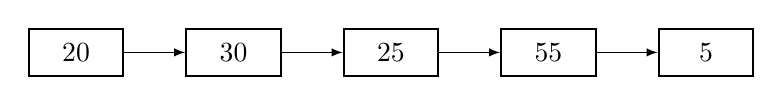
\begin{tikzpicture}[wagon/.style={minimum width=1.2cm,minimum height=0.6cm,draw,black,thick},
                    link/.style={-latex,thin},
                    address/.style={font=\tiny,circle,thin,fill=white}]

  \foreach[count=\i] \c in {20,30,25,55,5} {
    \pgfmathparse{(\i-1)*2}\let\x\pgfmathresult
    \node[wagon] (w\i) at (\x,0) {\c};
  }

  \foreach \i in {1,2,3,4} {
    \pgfmathparse{int(\i+1)}\let\j\pgfmathresult
    \draw[link] (w\i.east) -- (w\j.west);
  }
\end{tikzpicture}

\end{document}